% Document styling
\documentclass{article}
\marginparwidth 0.5in 
\oddsidemargin 0.25in 
\evensidemargin 0.25in 
\marginparsep 0.25in
\topmargin 0.25in 
\textwidth 6in \textheight 8 in

% List of packages
\usepackage[utf8]{inputenc}
\usepackage{fancyhdr}

% Custom paragraph indentation
\setlength{\parindent}{0em}
\setlength{\parskip}{1em}

% Packages for plots/images
\usepackage{graphicx}
\graphicspath{ {plots/} }
\usepackage{float}
\usepackage{subcaption}

% For appendix
\usepackage[toc, page]{appendix}

% SECTIONS
%
% * Report cover
% * Abstract
% * Sammanfattning
% * Table of contents
% * Introduction
% * Problem statement and purpose
% * Objectives
% * Social benefits, ethics and sustainable development
% * Outline
% * Background
% * Methodology
% * System
% * Results
% * Discussion
% * Conclusion
% * Limitations
% * APPENDIX: Additional figures
% * APPENDIX: Code location and running the experiment
% * Bibliography


\begin{document}


% ================================================== %
% == Report cover  == %
% ================================================== %

\title{
    \textbf{Experimental Methodology}\\
    \large{II1304 - Engineering Skills for ICT}
    }
\author{Cedric Seger and Simone Stefani}
\date{January 2018}
\maketitle
\thispagestyle{fancy}

\pagebreak

{\centering
\textit{This page intentionally left blank}\par
}
\pagebreak


% ================================================== %
% == Abstract == %
% ================================================== %

\section*{Abstract}
The task of executing actions with different level of priorities in a certain order is of fundamental importance in computer science and more broadly in most of the scientific disciplines. Priority queues (PQs) are data structures specifically designed for this purpose and can be implemented in different ways. In this paper we analyze two of these implementations, one based on a doubly linked-list and another based on a skew heap. We run a simulation of a workload on these two types of PQs in order to determine their performance in terms of speed. We consider also two types of setups: when a set of enqueue and dequeue operations are intermittently executed (HOLD method) and when a queue is first filled and then emptied (up-down method). The ultimate purpose of this experiment is to select the best implementation for a general purpose PQ with special focus on scheduling of processes or threads and future pending event sets in event-driven simulations. The two implementations are developed in C language and are executed multiple times with different data sets in order to included different cases and reduce the experimental error. While the performances may vary a lot based on the distribution of the input values, we determined that the skew heaps are substantially a better choice in case of large queues.

\pagebreak


% ================================================== %
% == Sammanfattning == %
% ================================================== %

\section*{Sammanfattning}
Uppgiften att genomföra åtgärder med olika prioritetsnivåer i en viss ordning är av grundläggande betydelse inom datavetenskap och i större utsträckning i de flesta vetenskapliga discipliner. Prioriterade köer (PQs) är datastrukturer som är speciellt utformade för detta ändamål och kan implementeras på olika sätt. I det här dokumentet analyserar vi två av dessa implementeringar, en baserad på en doubly linked-list och en annan baserad på en skew heap. Vi kör en simulering av en arbetsbelastning på dessa två typer av PQs för att bestämma deras prestanda när det gäller hastighet. Vi undersöker två typer av inställningar: när en uppsättning enqueue och dequeue-operationer utförs intermittent (HOLD-method) och när en kö fylls först och sedan töms (up-down method). Det ultimata syftet med detta experiment är att välja den bästa implementeringen för ett allmänt ändamål med särskild inriktning på schemaläggning av processer eller trådar och framtida pågående händelsessatser i händelsesdrivna simuleringar. De två implementationerna är utvecklade med hjälp av C och exekveras flera gånger med olika dataset för att inkludera olika fall och minska experimentfelet. Även om exekveringstiden kan variera mycket baserat på fördelningen av ingångsvärdena så visar resultaten att skew heaps är väsentligen ett bättre val vid stora köer.

\pagebreak


% ================================================== %
% == Table of contents == %
% ================================================== %

\tableofcontents

\pagebreak


% ================================================== %
% == Introduction == %
% ================================================== %

\section{Introduction}
Algorithms and data structures are at the heart of many technical inventions and innovations. They respectively provide a way to organize and manipulate data. However not every data structure is suitable for every kind of data and the same can be said about algorithms. Furthermore, even the same set of data may require to be manipulated in different ways depending on the purpose and circumstances. In reality algorithms and data structures are not two separate tools: they are often combined in order to provide dynamic and optimized solutions to common problems. The mathematical nature of these tools allows also for an in-depth analysis of performance and risks.

The problem of managing a queue where all the element have different levels of priority is quite common and easy to imagine. In the real life, citizens who reach an emergency department (ED) of an hospital receive different \textit{emergency codes} based on the severity of their conditions and are queued according to these. Similar necessities are quite common in the IT and software environment. In order to address this needs a specific data structure has been designed: the \textbf{priority queue}.

\pagebreak


% ================================================== %
% == Problem statement and purpose == %
% ================================================== %

\subsection{Problem statement and purpose}
The task of executing actions in a certain order is of paramount importance in computer science and more broadly in most of the scientific disciplines. One of the most common solution to this problem in the area of software engineering is to insert items in a queue data structure which can order them based on a given score. This data structure is called priority queue and it widely used, for example in scheduling of processes and in event-driven simulations.

Since priority queues can be implemented in very many different ways, it is fair to assume that there would be differences in functionality and efficiency among these implementations. Considering that so many systems relies on priority queues, it is obvious that choosing the most suitable implementation can both benefit in terms of precision and performance the underlying system. Hence the importance of performing a scientifically comparison between two priority queues, one using doubly linked-lists and the other using skew heaps.

\pagebreak


% ================================================== %
% == Objectives == %
% ================================================== %

\subsection{Objectives}
This report aims to investigate the execution time for two different implementations of priority queues. The two implementations to be compared are a skew heap and a doubly linked-list version. The C programming language has to be used for this task and the performances of the two versions of priority queues need to be accurately timed. The method of generating random items to be inserted in the queues needs to be carefully selected and justified.

The final evaluation should serve as a basis for choosing a priority queue implementation in general cases, therefore considering both analytic and execution best, worst and normal case performance. In particular the two needs that ought to be addressed are:

\begin{enumerate}
    \item scheduling queues for processes or threads with integer priorities in a limited range
    \item future pending event sets in event-driven simulations
\end{enumerate}

It is expected that, by the end of this study, a clear performance evaluation of the two implementation, based on the scientific method, will be available to the reader. 

\pagebreak


% ================================================== %
% == Social benefits, ethics and sustainable development == %
% ================================================== %

\subsection{Social benefits, ethics and sustainable development}
The most important benefit of an efficient implementation of a priority queue is a a fast and reliable performance of the application which makes use of it. For example operating systems can schedule more efficiently processes and thread operations, yielding a higher processing speed and consuming less energy.

On the ethical perspective the main concern regards safety and reliability of a higher level service. Since almost any device with a processor make use of PQs and many of the are at the core of our services, it is reasonable to think that a good implementation of the latter will ensure a correct behavior of such devices.

\pagebreak


% ================================================== %
% == Outline == %
% ================================================== %

\subsection{Outline}
In section 2, \textit{Background}, the key topics used in this assignment are introduced, starting from the main data structures: binary heap, skew heap and doubly linked-list. After that two use cases for PQs are briefly described in  sections 2.2 and 2.3. In section 3 we explain which process and methodologies are used for data collection and analysis and we define some validation criteria used to determine the correctness of implementation and consistency of results (section 3.3). Section 4 analyzes the structure of the implementation from a purely technical perspective and the experimental setup for the simulation. Finally, in section 5, the result of the experiments are presented and conclusions are drawn.

\pagebreak


% ================================================== %
% == Background == %
% ================================================== %

\section{Background}

\subsection{Priority queues}
There is often a need in applications to process objects sequentially in some order related to their priority, while it is not necessary to have all items completely sorted. Priority queues solve this problem and represent a fundamentally important data structure in computer science. PQs are typically used as a building block in larger, more complex applications and algorithms. An operating system could, for example, make use of a PQ in order to choose the next process to run. Another example is the use of PQs in graph algorithms, Dijkstra, compression algorithms and sorting such as heapsort \cite{sedgewick}.

These examples also highlight the functions that a PQ must support. At its most basic level, a PQ implementations provide methods for removing the maximum element in a queue and for inserting new elements into the queue. The efficiency of these operations, therefore, are what determines the efficiency of a PQ and will vary widely depending on the actual implementation. A brief overview of the type of possible implementations will be given next.

\subsubsection{Binary heap}
The classical PQ implementation is the binary heap. The binary heap stores items in a binary tree where each parent node's key is larger than or equal to each of the keys belonging to its two children nodes. The actual implementation is, however, based on an array in which parent and children nodes are a multiple of two and two plus one apart \cite{sedgewick}. This allows for simple index arithmetic to efficiently travel up and down the heap. The root node of the heap is the one with the greatest key or least key if it is a min-heap. The efficiency of the binary heap implementation comes from the fact that the height of a binary tree of size \(N\) is no greater than \(lg N\). This has the implication that the worst case scenario for insertion and popping operations is guaranteed to be \(O(lg N)\).

\subsubsection{Skew heaps} \label{heapbackground}
The skew heap, also known as a self adjusting binary heap, was first introduced by Sleator and Tarjan \cite{sleator}. They introduced the idea of optimizing the efficiency of a PQ with respect to its amortizing costs over several operations. This is unlike other PQ implementations, such as the binary heap, that focus on achieving the lowest worst-case time penalty on a per operation basis. The problem of these classical algorithms, however, are that they achieve this only by introducing specific structural constraints that must be maintained at all times. Instead, a skew heap does not impose any explicit structural constraints but allow for the insertion and popping operations to modify the structure in a simple way.

The characteristic operation of a skew heap is its meld operation, which takes two disjoint heaps and combine them into one. This operation works by traversing the right-most paths of each tree and merging them into a single right path in increasing order. The left paths of the nodes along the merge path do not change. Other important operations such as delete and insertion make use of the meld operation. Specifically, an insert(node, tree) turns the node into a single one-node tree and melds it with the existing tree. The delete min(node) operation works by replacing the node in the tree by the meld of its left and right subtrees.

It is therefore critical that the meld operation is efficient. This is guaranteed if the right-most path is kept short as the meld operation has a time complexity linearly related to the length of the merge path. The skew heap tries to do so by swapping the left and right children, except the lowest, on the merge path after a meld operation has been done. This avoids the long right path problem by making them into left paths. Following this algorithm, it guarantees an \(O(lg N)\) amortized bound on any operations performed on the skew heap, where n is the number of items in the heap or the number of heaps involved in an operation.

The disadvantage with skew heaps is that the worst-case cost per operation can remain large. It is possible to construct sequences in which a particular operation would take \(O(n)\) time. This could cause problems for realtime applications that need to respond quickly for each operation.

\subsubsection{Doubly linked-lists} \label{listbackground}
In order to improve the performance of this data structure when it is needed to operate on the tail, it is common practice to store a link in every node to the previous one and to keep track of the \textit{tail} together with the \textit{head}. Hence the name \textit{doubly linked-list}.

A doubly linked-list can be used to implement a priority queue. In such case every node contains also a priority index. Here it is possible to make decisions about the design of the priority queue; for the purpose of this report we assume that a new node is enqueued and positioned in the correct priority order with highest priority index at the head of the queue. The insertion of a new node occurs from the front if the priority of the new node is higher than the average of the priorities of the first and last nodes in the list, otherwise the insertion will occur from the end of the list. A dequeue operation consist in removing the first element of the list and setting the second node as head.
It is then clear that an insertion operation requires to traverse the list until the correct priority position is found. If we assume a normal distribution of priority indexes we can expect that an insert operation will require to traverse on average a quarter of the list and consequently will have a complexity $O(\frac{n}{4}) \sim O(n)$. The best case will result when any new node that needs to be inserted has priority either greater or smaller than any other node already present in the list; in such situation the insertion complexity is $O(1)$. The worst case happens when an element needs to be inserted in the middle of the list and the complexity for such operation is $O(\frac{n}{2}) \sim O(n)$.

On the other hand dequeueing an element from the list is a simple operation and involves only manipulation of the tail which is easily accessible, yielding a time complexity of $O(1)$ for best, average and worst case.

\subsection{Event driven simulation}
In developing scientific applications, simulation techniques are often employed in order to understand certain phenomena better. This is immensely useful in situations in which an analytic approach is either intractable or too difficult. One can, for example, model the motion of of a system of moving particles using an event-driven simulation approach.

In event-driven simulations the key operations to be executed are the scheduling of future events and the execution of the next pending event \cite{vaucher, McCormack}. These respectively correspond to inserting an item of arbitrary priority into a data structure and removing the item with the highest. As an aside, it is common practice to schedule events with identical priority in terms of a first-in-first-out (FIFO) order. It is clear that the data structure that implements these operations lends itself nicely to the idea of a priority queue.

The main interest then becomes to choose a priority queue that implements insertion and deletion operations efficiently as this is crucial to the execution time of a simulation. Particularly for large models, the overhead incurred by these operations tend to account for a major part of a program's running time \cite{vaucher}. While speed is important, it is also critical that the implementation is robust. This refers to that the running time of these operations must be maintained under a wide range of running conditions.

\subsection{Process and thread scheduling}
Process and thread scheduling is one of the main task of every operating system. The topic of scheduling is very broad and multiple scheduling techniques are used in order to achieve performance \cite{coffman1968computer}. In fact an OS which is able to efficiently schedule process making use of the available resources will definitely show improvements in speed compared with a system which implements a naïve scheduler.

It is also relevant to mention that scheduling involves a reliability component. In fact high-volume and ill-behaved applications may overtake the available computational power of a machine if the OS is not able to strategically determine how attribute priorities to different processes.

From these two brief points on the purpose and requirements of a process scheduler it is reasonable to think that priority queues can be a suitable data structure to manage scheduling. In this scenario the scheduler is responsible of attributing a priority value to each item and to enqueue it. Every time the processor is available the scheduler pops an element from the queue which result to have highest priority.

It is important to keep in mind that the implementation of queue-based scheduler in an OS can be very complicated and involves a large number of different strategies and also multiple queues which handle different priorities ranges \cite{arzen2000introduction}.\\
Moreover in the simple implementation for this task the priorities will be described by a small range of non-negative integers.

\pagebreak

\subsection{Related work}
There has been several studies that investigate the timing complexity of priority queues in relation to event simulation models. One of the most notable is the work done by Jones \cite{Jones}, who studied the execution times of priority-queue implementations under a hold model. The study shows that skew heaps performs better than implicit heaps and has similar performance to pairing heaps and pagodas. Further, it is indicated that skew heaps are one of the simplest priority queues to implement and remain relatively insensitive to changes in the priority distribution used for scheduling new events. Simple linked-lists remain the best implementation for fewer than 10 items in the queue. Vaucher and Duval \cite{vaucher} compared linear list, tree-based and indexed list algorithms and found indexed lists performed best. Interestingly, the authors made use of six different, stochastic distributions, representative of various kinds of simulation problems, to test the running times of the algorithms, also using the HOLD method. McCormack \cite{McCormack} is one of the few studies that present analytic reasoning and results for the use of the HOLD model in event simulation and provides a thorough empirical testing of 12 different priority queues. In addition, it is pointed out that care must be taken when using the HOLD model. In real simulations, events are often scheduled by more than one distribution and as a result there is an increase in the probability that new insertions will have a smaller due-time than those already in the future event set.

\pagebreak


% ================================================== %
% == Methodology == %
% ================================================== %

\section{Methodology}

\subsection{Considerations}
In this assignment we are going to make use of a general version of the scientific experimental method. Thanks to the literature study, whose results are briefly summarized in \textit{Background} section, it is possible to formulate some hypothesis on the compared performances of the two implementations of the priority queues.

After that, a set of experiments should be arranged. The two implementations of PQs needs to be realized into C code keeping in mind the requirements. Then, for the purpose of the experimental simulation, two different aspects should be carefully considered:

\begin{enumerate}
    \item generation of random data and priority values
    \item timing functions
\end{enumerate}

When generating random data one should first of all consider a suitable pseudo-random number generator. This involves consulting and comparing documentation and specifications of different tools which may be available.
Secondly the quality of the generated value should be evaluated together with the final purpose of the priority queues. For a general use some sort of normally distributed set if integers may be a good solution while for a use as process scheduler it may be appropriate to generate small unsigned integers. Finally for the event-driven simulation the priorities are represented as virtually unlimited timestamps.

For the timing of the PQs functions one must pay attention to the what operations are included or excluded from the timed code block. Furthermore a main choice needs to be made if to measure execution time of single calls or aggregated groups of calls. While the first possibility may seem easier, it also carry a risk of higher imprecision since some fixed errors may weight more than in reality. The second possibility also allows for amortized analysis.

While the task is all about measuring the time efficiency of different implementation of priority queues, it can also be useful to track the memory usage. This can in fact become an obstacle and a prominent criteria in the selection of an implementation for a specific purpose.

\subsection{Choice of methods}
From the literature and background study it is clear that the speed of operations carried out on a priority queue will depend on several parameters. For example, the number of elements in the queue, the distribution of the elements in the queue, the sequence in which operations are performed and the distribution of elements to be enqueue. For these reasons and with reference to previous studies, \cite{Jones, McCormack, vaucher}, the evaluation of the usage of priority queues is done using a hold model.

The hold model is appropriate as it facilitates the measurement of the average execution time per operation over longer sequences of operations. It also allows for direct comparisons of how the queue implementations vary with changing queue size. Specifically, a hold operation is specified as a dequeue followed by an enqueue operation and hence keeps the queue size fixed during testing. Further we choose to use seven different priority distributions to test the behaviour of the algorithms under varying conditions. In particular, the following distributions were chosen:

\begin{enumerate}
    \item Negative Exponential with \(\lambda = 1\)
    \item Continous Uniform \(interval \in [0, 2]\)
    \item Continous Uniform \(interval \in [0.9, 1.1]\)
    \item Triangular \(0.5rand^{0.5}\)
    \item Constant \(Value = 1\)
    \item Discrete with uniform probability \(interval \in [1-5]\)
    \item Compound (distribution1, distribution2, N)
\end{enumerate}

These distributions were chosen due to their different characteristics and representation of actual problems \cite{vaucher}. Further, as mentioned by McCormack \cite{McCormack}, and hinted by Robert \cite{Ronngren}, actual scheduling of events do not typically follow the same distribution. Scheduling of events often depend on more than one distribution and for this reason chose to include a compound distribution as well. The compound distribution combines two arbitrary distributions in which \(N\) draws from one distribution are concatenated with \(N\) draws from the other. In order for a fair comparison between the two queue implementations, a trace of all enqueue operations to be made were computed and stored before running the hold operations. Moreover, this reduces the costs of each test.

Following similar style to Jones \cite{Jones}, all timing measurements are made over a sequence of 1000 operations in order to reduce the effect overhead on measurement error. Also, 500 trials for each measurement were conducted over a range of queue sizes in range (10,5000).

\subsection{Validation of method, setup and results}
The experiment described in this report runs in a closed box; our setup and implementations allow to generate measurements regarding the operational times of two different implementation of priority queues with several inputs and parameters. However they do not convey any information regarding the correctness of the implementations, the consistency of the results or the suitability of the setup. For this reasons it is fundamental to invest energies into a simple but well thought validation process.

There are two main areas where the experiment requires validation:

\begin{enumerate}
    \item Correctness of implementation of the data structures (linked-list and skew heap)
    \item Consistency in the collected results
\end{enumerate}

\subsubsection{Correctness of implementation}
In order to validate the implementation of the data structures, an approach based on integration testing is used. This is a form of black-box testing since there is no complete awareness on the internal implementation of the data structures but some exposed methods are used in combination with known data to verify that expected results are obtained. Since both the data structures expose a similar API, they are also tested in a very similar way. Here are listed some basic test cases for the doubly linked-list PQ (same methods are used for the skew heap):

\begin{itemize}
    \item \texttt{test\_enqueue\_list}: test if the linked-list can correctly enqueue a new element and hence grows in size of one.
    \item \texttt{test\_dequeue\_list}: test if the linked-list can correctly dequeue an element and hence decrease in size of one.
    \item \texttt{test\_reset\_list}: test if the linked-list can be correctly reset, i.e. all elements are removed.
    \item \texttt{test\_dequeue\_smallest\_element}: test if the \texttt{dequeue()} methods returns the smallest element in the list, i.e. the element with highest priority.
    \item \texttt{test\_queue\_maintains\_internal\_order}: test if the list maintains a correct internal order of the elements based on priority. In such case, in a sequence of dequeue operations, every dequeued element should be smaller (i.e. has higher priority) than the element previously dequeued.
\end{itemize}

These five simple test cases are enough to determine if the implemented data structures behave correctly.

The tests have been written as simple functions which make use of the basic C \texttt{assert()} library. While more advanced testing frameworks such as Check and CUnit are avaiable, they would have only caused a complex implementation totally disproportionate compared to the simple task of this experiment.

\subsubsection{Consistency in results}
The second major goal of validation in this project is to verify that the collected data has an internal consistency and reflect realistic outcomes. This means that the time values must be positive numbers and that by increasing the amount of operations (enqueue and dequeue) while keeping other parameters fixed, the measured times would also increase yielding bigger numbers.
Furthermore, during the background research, some estimates of the time complexity of operations have been described (sections \ref{heapbackground} and \ref{listbackground}). Hereby it is possible to run the experiment with data structures of varying size and evaluate if the results are consistent with the pre-determined time complexity within reasonable consistency intervals. 

On a more general level, plotting graphs is useful technique to spot anomalies in the collected data. The anomalies are not necessarily a sign of an error or a bug, but can help to direct the investigation towards sources of possible problems. These types of validation can be conducted after the results have been collected.

\pagebreak


% ================================================== %
% == System == %
% ================================================== %

\section{System}

\subsection{System development method}
The system to carry on this experiment has been built on top of several different technologies. The reason of this decision is that different tools work better for different purposes. Furthermore is very likely that a person is more skilled in a programming language or paradigm than in another. Hence the choice of tools upon which building the system results to be a compromise between the customer requirements and the knowledge of the involved people.

As per requirements, the PQs data structures are implemented in C language since it provides a simple environment where performance testing does not risk to be influenced by further decorative features. The C files are then compiled with the traditional Gnu C Compiler (GCC). Input and output data is read or written to plain text files.

The input data is generated according to specific distributions by a Python script. Another Python script is used to analyze the output data and plot suitable graphs using the renown libraries \texttt{matplotlib} and \texttt{seaborn}. The choice of Python against something more traditional like GNUPlot is due to the fact that Python script environment is more dynamic and requires a shortest setup time. It also comes with a larger and more active community.

\subsection{Implementation structure}
In general, the code base tends to have a modular structure: the data structures expose a very similar API which is called by a main \textit{runner function}. Such function is then called by a Python script which uses different arguments, passing input data and collecting the output.

The data structures expose the following functions:

\begin{itemize}
    \item \texttt{enqueue\_heap} and \texttt{enqueue\_list}: add a new element to the data structure.
    \item \texttt{dequeue\_heap} and \texttt{dequeue\_list}: remove the element with highest priority from the data structure.
    \item \texttt{reset\_heap} and \texttt{reset\_list}: remove every element from the data structure and free the allocated memory.
    \item \texttt{count\_heap\_elements} and \texttt{count\_list\_elements}: return the number of element in the data structure.
\end{itemize}

These methods are used both for purpose of running the experiment and for testing. The file \texttt{main.c} contains the main method to run the experiment; it accepts a set of arguments and saves the results in CSV files. The following arguments are accepted from the main function:

\begin{itemize}
    \item \texttt{-i <heap|list>}: the type of data structure on which run the experiment. \texttt{list} is the default option.
    \item \texttt{-q <size>}: the initial size of the queue. Default 0.
    \item \texttt{-h <0|1>}: the chosen simulation method, 0 for \textit{up-down} and 1 for \textit{hold}. Default 1 (\textit{hold}).
    \item \texttt{-d <input-path>}: the path to the input text files.
    \item \texttt{-s <output-path>}: the path for the output files.
    \item \texttt{-o <operations>}: number of enqueue and dequeue operations to execute inside a timed interval. Default 0.
    \item \texttt{-t <trials>}: number of repeated trials where a certain number of operations are timed. Default 0.
\end{itemize}

A sample command can be:

\begin{verbatim}
./a.out -i heap -q 10 -h 1 -d samples/triangular.txt -s out/triangular.csv -o 100 -t 5   
\end{verbatim}

In order to execute this command more easily on all the different data distributions described in the previous sections and on the two distinct data structures, a Python runner script \texttt{task\_runner.py} has been created. However it requires Python 3.5 or higher to work. If this requirement is fulfilled it will suffice to run the following command to execute the whole experiment on all the available inputs:

\begin{verbatim}
python3 task_runner.py 
\end{verbatim}

The file \texttt{input.c} exposes methods to read the input files and write output CSV files, while \texttt{Distribution Generator.ipynb} contains Python functions to generate distributions and plots inside a Jupiter Notebook.

\subsection{Experimental setup and data collection}
For ease of execution the experiment was run on a personal laptop MacBook Air Mid-2013 with a 1,3GHz Intel Core i5 processor and 4GB of 1600 MHz DDR3 RAM. The experiment has been executed 500 times with 1000 operations each in order to reduce the error introduced by external factors such other processes running on the same machine.

The results of the experiment are written to file as comma-separated values (CSV) for further analysis and manipulation. By not sending the data directly to a \textit{processing pipeline} we allow for greater flexibility since we can then use different tools to perform specific and accurate analysis. In particular, Python with numpy and matplotlib packages was used for data post-processing during which we calculated the mean and standard deviation of the 500 trials, for each experiment conducted. All graphs were then plotted with the mean execution time as the dependent variable and queue size as the independent variable. Error bars were shown by plotting one standard deviation for each calculated mean.

For a list of the actual distributions used in the experiments, please refer to figure \ref{fig:distributions_used} in the appendix.

\pagebreak


% ================================================== %
% == Results == %
% ================================================== %

\section{Results}
This section describes the results obtained from the experiments.

\subsection{Across priority distributions}
\begin{figure}[H]
\centering
    \begin{subfigure}[H]{0.4\linewidth}
    \includegraphics[width=\linewidth]{Execution_time_for_heap:hold=1.png}
    \caption{Hold method: heap}
    \label{exec_heap_hold}
    \end{subfigure}
    \begin{subfigure}[H]{0.4\linewidth}
    \includegraphics[width=\linewidth]{Execution_time_for_heap:hold=0.png}
    \caption{Up-down method: heap}
    \label{heap_up_down_first}
    \end{subfigure}
    \begin{subfigure}[H]{0.4\linewidth}
    \includegraphics[width=\linewidth]{Execution_time_for_list:hold=1.png}
    \caption{Hold method: list}
    \end{subfigure}
    \begin{subfigure}[H]{0.4\linewidth}
    \includegraphics[width=\linewidth]{Execution_time_for_list:hold=0.png}
    \caption{Up-down method: list}
    \label{}
    \end{subfigure}
\caption{Execution times for heap and list}
\label{fig:heap_list_exec}
\end{figure}

From figure \ref{fig:heap_list_exec} it is evident that the type of priority distribution used has a clear impact on the execution time for both skew heaps and linked-lists. The impact is most clearly seen for larger queue sizes while for smaller queue sizes the type of priority distribution becomes less significant, with execution time converging towards zero. Linked-lists have a more kinked convergence than heap and large differences start to show for queue sizes larger than 1000 elements.

Analyzing further, both linked-lists and heaps generally experiences best performance for the constant and categorical priority distributions. Similarly, when using the hold method, both data structures performed worst with priority distributions such as triangular, exponential and uniform, with the addition that skew heap also performed badly on the compound distribution. For up-down method the list data structure experienced worst performance with compound and exponential distributions and middle performance on the the triangular, uniform and categorical ones. Similar behaviour is shown for the skew heap.

Also of interest is the size of the error bars, particularly for figure \ref{heap_up_down_first} and \ref{exec_heap_hold}. In both of these experiments, the error bars, or the spread of the data, becomes relatively large for bigger queue sizes.

\subsection{Across data structure}
\begin{figure}[H]
\centering
    \begin{subfigure}[H]{0.4\linewidth}
    \includegraphics[width=\linewidth]{HeapvsList:hold=1_dist=exponential_samples.png}
    \caption{Heap vs. List: Exponential Distribution, hold}
    \label{fig:heap_vs_list_expo}
    \end{subfigure}
    \begin{subfigure}[H]{0.4\linewidth}
    \includegraphics[width=\linewidth]{HeapvsList:hold=1_dist=constant_1.png}
    \caption{Heap vs. List: Constant Distribution, hold}
    \label{fig:heap_vs_list_const_hold}
    \end{subfigure}
    \begin{subfigure}[H]{0.4\linewidth}
    \includegraphics[width=\linewidth]{HeapvsList:hold=0_dist=constant_1.png}
    \caption{Heap vs. List: Constant Distribution, up-down}
    \label{fig:heap_vs_list_const}
    \end{subfigure}
\caption{Heap vs. List}
\label{fig:heap_vs_list}
\end{figure}

Although skew heaps and linked-lists are similarly affected by the type of priority distribution, the results in figure \ref{fig:heap_vs_list_expo} clearly show that skew heaps have a much faster execution time than linked-lists for the exponential distribution. This relationship holds for all the other distributions as well, as seen from figure \ref{fig:heap_vs_list:appendix} in appendix, except for the constant distribution as evident in figures \ref{fig:heap_vs_list_const} and \ref{fig:heap_vs_list_const_hold}. For the constant distribution, lists and heaps performed, approximately, equally well.

\subsection{Across experiment method}
\begin{figure}[H]
\centering
    \begin{subfigure}[H]{0.4\linewidth}
    \includegraphics[width=\linewidth]{HoldvsNo-Holdforheap.png}
    \caption{Hold vs. up-down: heap}
    \label{}
    \end{subfigure}
    \begin{subfigure}[H]{0.4\linewidth}
    \includegraphics[width=\linewidth]{HoldvsNo-Holdforlist.png}
    \caption{Hold vs. up-down: list}
    \label{}
    \end{subfigure}
\caption{Hold vs. up-down}
\label{fig:hold_vs_no_hold}
\end{figure}

Further interesting is how the two data structures perform generally against hold operations versus up-down operations. Figure \ref{fig:hold_vs_no_hold} shows that hold operations are more expensive for both heaps and lists for queue sizes greater or equal to 1000. For smaller queue sizes this effect is less dramatic.


% ================================================== %
% == Discussion == %
% ================================================== %

\section{Discussion}
As evident from the results section, it is clear that the skewed heap version of the priority queue is much faster than the linked list version in the general case for queue sizes larger than 1000. For smaller queue sizes the type of implementation matters less. These results are also supported analytically. The skew heap has a guarantee for \(O(lg N)\) amortized time complexity for any one operation, whereas the doubly linked-list has a time complexity of approximately \(O(n)\) for insertions and \(O(1)\) for dequeues. Hence for any larger amount of operations that involve both insertions and dequeues, the \(O(n)\) complexity of the linked-list quickly outweighs its benefit of constant time complexity for dequeues.

The exception to this rule is when the implementations operate under a constant distribution of ones. For the linked-list this type of distribution will cause it to constantly insert at the tail and popping from the head of the list, both of which are constant time operations. For the skew heap insertions will still traverse the entire right hand side of the tree but since the right hand side is kept short, the heap performs well.


% ================================================== %
% == Conclusion == %
% ================================================== %

\section{Conclusion}
The aim of this report was to investigate the execution time for two different implementations for priority queues, namely a skewed heap implementation and a doubly linked-list version. The purpose of this evaluation was to serve as a basis for choosing a priority queue implementation in the general case, in particular for event-driven simulations and process scheduling.

To this end, it seems that the skewed heap implementation of the priority queue will serve as the best general implementation when compared to a doubly linked-list version. This is particularly true when considering event-driven simulations, for which the total time of executing numerous simulations is of importance. For real-time applications in which any one single operation may be important, the skewed heap, however, does not offer any guarantees.


% ================================================== %
% == Limitations == %
% ================================================== %

\section{Limitations}
This report did not investigate execution times for queue sizes larger than 5000. This meant that the execution times for 1000 operations on the queues, although significantly different, remained relatively small. It would be interesting to investigate if similar relationships hold for larger queue sizes. Also, the experiments were carried out on a personal laptop. This inevitably means that uncertainty in the measurements increase since the OS can choose to schedule other operations at the same time. To make measurements more accurate one could make use of special purpose hardware that does not run other programs. Additionally, it is possible to make more trials of each experiment than the 500 used in this report. This would increase the robustness of the results.

\pagebreak


% ================================================== %
% == APPENDICES == %
% ================================================== %

\appendix


% ================================================== %
% == Additional figures == %
% ================================================== %

\section{Additional Figures}

\begin{figure}[H]
\centering
    \begin{subfigure}[H]{0.4\linewidth}
    \includegraphics[width=\linewidth]{HeapvsList:hold=1_dist=categorical_5.png}
    \caption{Heap vs. List: Categorical Distribution, hold}
    \end{subfigure}
    \begin{subfigure}[H]{0.4\linewidth}
    \includegraphics[width=\linewidth]{HeapvsList:hold=1_dist=triangular.png}
    \caption{Heap vs. List: Triangular Distribution, hold}
    \end{subfigure}
    \begin{subfigure}[H]{0.4\linewidth}
    \includegraphics[width=\linewidth]{HeapvsList:hold=1_dist=uniform_samples.png}
    \caption{Heap vs. List: Uniform Distribution, hold}
    \end{subfigure}
    \begin{subfigure}[H]{0.4\linewidth}
    \includegraphics[width=\linewidth]{HeapvsList:hold=1_dist=uniform_samples_limited.png}
    \caption{Heap vs. List: Uniform Limited Distribution, hold}
    \end{subfigure}
    \begin{subfigure}[H]{0.4\linewidth}
    \includegraphics[width=\linewidth]{HeapvsList:hold=1_dist=compound.png}
    \caption{Heap vs. List: Compound Distribution, hold}
    \end{subfigure}
\caption{Heap vs. List: Appendix}
\label{fig:heap_vs_list:appendix}
\end{figure}

\begin{figure}[H]
\centering
    \begin{subfigure}[H]{0.8\linewidth}
    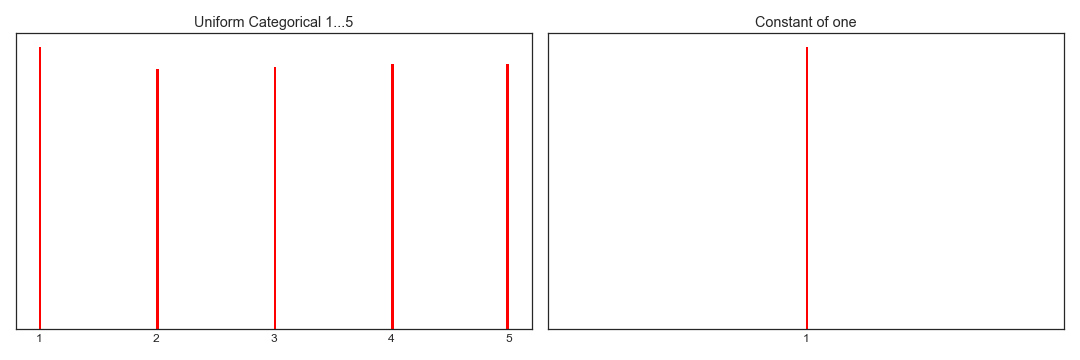
\includegraphics[width=\linewidth]{input_distributions_cat.png}
    \caption{Categorical Distributions}
    \end{subfigure}
    \begin{subfigure}[H]{0.8\linewidth}
    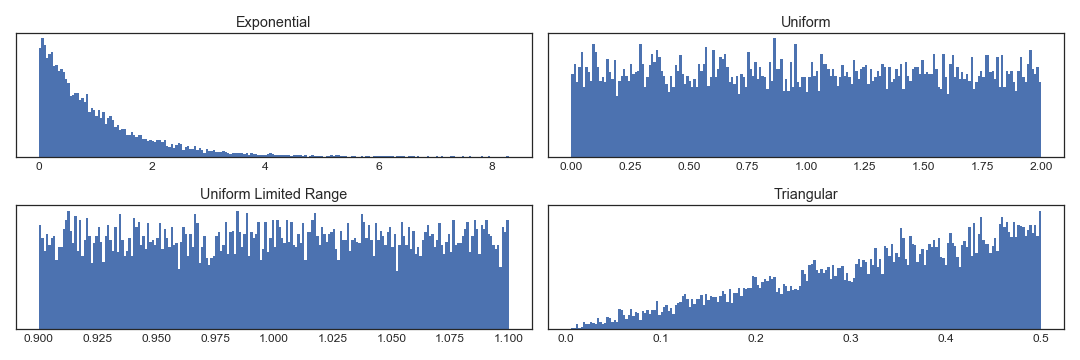
\includegraphics[width=\linewidth]{input_distributions_cont.png}
    \caption{Continuous Distributions}
    \end{subfigure}
\caption{Distributions used in experiments: Appendix}
\label{fig:distributions_used}
\end{figure}

\pagebreak


% ================================================== %
% == Code location and running the experiment == %
% ================================================== %

\section{Code location and running the experiment}

\subsection*{Location of the Source Code}
The code has been uploaded to the KTH AFS through the server \texttt{u-shell.csc.kth.se}.\\\\ The location of the simulation files is: \texttt{/home/s/s/sstefani/priority-queues}

\subsection*{Source code and raw data}
Considering the length of the source code and the quantity of produced raw data we have decided to refer to an external repository located on GitHub. This approach is also becoming more common in the broad academical environment due to its simplicity.

The address of the repository is: \url{https://github.com/SimoneStefani/priority-queues}

The data structure implementation code can be specifically found in this sub-folder together with the test code: \url{https://github.com/SimoneStefani/priority-queues/tree/master/src}

The raw data from a sample simulation is available in this sub-folder:
\url{https://github.com/SimoneStefani/priority-queues/tree/master/output}

The graphs derived from the raw data are available in this sub-folder:
\url{https://github.com/SimoneStefani/priority-queues/tree/master/plots}

\subsection*{Running the experiment}
In order to run the experiment with custom parameters first compile the C files in \texttt{src/}:

\begin{verbatim}
$ cd src/
$ gcc input.c linked_list_pq.c main.c skewed_heap_pq.c -o experiment.out   
\end{verbatim}

Then run the executable:
\begin{verbatim}
$ ./experiment.out
\end{verbatim}

Check section 4.2 for more information on the parameters.

Example input:

\begin{verbatim}
$ ./experiment.out -i heap -q 10 -h 1 -d samples/triangular.txt -s samples/triangular_exec -o 100 -t 5
\end{verbatim}

\subsubsection*{Running the Python script}
This feature requires Python 3.5 or greater on the machine. In the main base folder run:

\begin{verbatim}
$ python3 task_runner.py
\end{verbatim}

\subsubsection*{Running the tests}
Move in the \texttt{src/} folder compile the test with the corresponding data structure implementation and run the executable:
\begin{verbatim}
$ cd src/
$ gcc linked_list_pq.c linked_list_pq_test.c -o linked_list_test.out
$ ./linked_list_test.out
\end{verbatim}

\pagebreak


% ================================================== %
% == BIBLIOGRAPHY == %
% ================================================== %

\bibliographystyle{IEEEtran}
\bibliography{references}

\end{document}
